%------------------------------------------------------------------------------
\chapter{Hohlraumresonatoren}
\label{sec:hohlraumresonatoren}
%------------------------------------------------------------------------------


%------------------------------------------------------------------------------
\section{Elektromagnetische Felder in Hohlraumresonatoren}
%------------------------------------------------------------------------------
Ein Hohlraumresonator besteht aus einem (i.\ d.\ R.\ evakuierten) Hohlraum, welcher durch ein leitendes Material begrenzt wird.
Im Hohlraum propagierende elektromagnetische Wellen werden an den leitenden Wänden reflektiert und führen zur Ausbildung von stehenden elektromagnetischen Wellen im Resonatorinnenraum, welche unter anderem zur Beschleunigung von elektrisch geladenen Teilchen genutzt werden können.
Aufgrund der Randbedingungen an der näherungsweise ideal leitenden Grenzfläche müssen die folgenden Anforderungen an das elektromagnetische Feld gestellt werden:
\begin{align}
  E_\parallel = 0 \qquad \text{und} \qquad B_\perp = 0 \eqcomma
  \label{eq:randbedingung_leiter}
\end{align}
wobei $E_\parallel$ die Tangentialkomponente und $B_\perp$ die Normalkomponente des elektrischen bzw.\ magnetischen Feldes auf der Grenzfläche kennzeichnet.
Die Lösung der \textsc{Maxwell}-Gleichungen unter Beachtung dieser Randbedingungen zeigt, dass eine unbegrenzte Anzahl von Schwingungsmoden der stehenden Welle im Resonator auftreten können.
Jede dieser Moden besitzt eine charakteristische Eigenfrequenz, die von der Hohlraumgeometrie abhängig ist. 
Die Klassifizierung der einzelnen Moden erfolgt anhand ihrer Feldkonfiguration relativ zur Propagationsrichtung der hin- und rücklaufenden Wellen im Resonator.
Dabei unterscheidet man zwischen transversal-elektrischen (TE)-Moden, welche lediglich transversale elektrische und longitudinale magnetische Felder aufweisen und transversal-magnetischen (TM)-Moden, bei denen der umgekehrte Fall vorliegt.

Viele der in Beschleunigern verwendeten Kavitäten\footnote{von lat.\ \emph{cavum} \glqq Höhle\grqq: Hohlraumresonator oftmals engl. \emph{Cavity}} basieren auf kreiszylindrischen Resonatoren\footnote{engl. \emph{Pillbox-Cavities}, für deren Ähnlichkeit mit einer Tablettenschachtel}.
Diese erlauben eine analytische Lösung der \textsc{Maxwell}-Gleichungen.
Daher soll im Folgenden die Feldkonfiguration der verschiedenen Moden in einem solchen Resonator dargestellt werden und die in dieser Arbeit verwendete Notation eingeführt werden.
Dabei genügt die Betrachtung der longitudinalen Felder eines zylindrischen Hohlraums mit Radius~$R$ und Länge~$L$ in Zylinderkoordinaten~$(r \in [0, R], \theta \in [0,2\pi), z \in [0, L])$, da durch diese die transversalen Feldkomponenten eindeutig festgelegt sind \cite[S.\ 4]{hillert}.
Man findet für die Moden in dem kreiszylindrischen Resonator \cite[S. 28 ff.]{wangler}:
\begin{subequations}
  \begin{align}
  \mathrm{TM}_{mnp}\text{-Mode:}& \quad &E_z = E_0 J_m(k_{mn} r) \cos(m \theta) \cos\left(\frac{p \pi z}{L}\right) \exp(\I \omega_{mnp} t) \eqcomma \qquad B_z &= 0\\
  \mathrm{TE}_{mnp}\text{-Mode:}& \quad &B_z = B_0 J_m(k_{mn}^\prime r) \cos(m \theta) \sin\left(\frac{p \pi z}{L}\right) \exp(\I \omega_{mnp}^\prime t) \eqcomma \qquad  E_z &= 0 \eqdot
  \end{align}
  \label{eqs:felder_pillbox}
\end{subequations}
Die Konstante $k_{mn}^{(\prime)}$ ist hierbei als
\begin{align}
k_{mn}^{(\prime)} := \frac{x_{mn}^{(\prime)}}{R}
\end{align}
mit der $n$-ten positiven Nullstelle $x_{mn}$ der Besselfunktion $m$-ter Ordnung $J_m(x)$ respektive ihrer Ableitung $J_m^\prime(x)$ definiert.
Aus den Gleichungen \eqref{eqs:felder_pillbox} folgt dann die Bedeutung der Indizes~$m, n$ und $p$:
Der Index $m$ ($m=0, 1, \dots$) beschreibt die Periodenzahl der Feldkomponente in azimutaler Richtung.
Weiterhin wird durch $n$ ($n=1, 2, \dots$) die Anzahl der Knoten der longitudinalen Feldkomponente in radialer Richtung (ausgenommen Knoten im Ursprung mit $r=0$) angegeben.
Schließlich gibt der Index $p$ (TM-Mode: $p= 0, 1, \dots$; TE-Mode: $p = 1, 2, \dots$) die Anzahl der halben Perioden in longitudinaler Richtung an.
Die Resonanzfrequenz~$\omega_{mnp}$ der einzelnen Moden ist dabei gegeben durch \cite[S.\ 28 ff.]{wangler}:
\begin{align}
\omega_{mnp}^{(\prime)} = c \cdot \sqrt{\left( k_{mn}^{(\prime)}\right)^2 + \left( \frac{p \pi}{L} \right)^2} \eqdot
\label{eq:frequenz_pillbox}
\end{align}
Die Gleichungen \eqref{eqs:felder_pillbox} und \eqref{eq:frequenz_pillbox} gelten für den Idealfall geschlossener zylindrischer Resonatoren und beinhalten daher keinen Eintritts-/Austrittsfenster für geladene Teilchen.
In der Praxis werden komplexere Resonatorgeometrien verwendet, für die eine analytische Berechnung der Eigenmoden im Allgemeinen nicht mehr möglich ist und auf numerische Methoden zurückgegriffen werden muss.
Dazu wird in dieser Arbeit \emph{CST Microwave Studio\textsuperscript{\textregistered}} verwendet, welches die Lösung der Maxwell-Gleichungen diskretisiert und auf ein Eigenwertproblem zurückführt.


%------------------------------------------------------------------------------
\section{Kenngrößen von Resonatoren am Modell des RLC-Parallelkreises}
%------------------------------------------------------------------------------
\begin{figure}[htb]
  \centering
  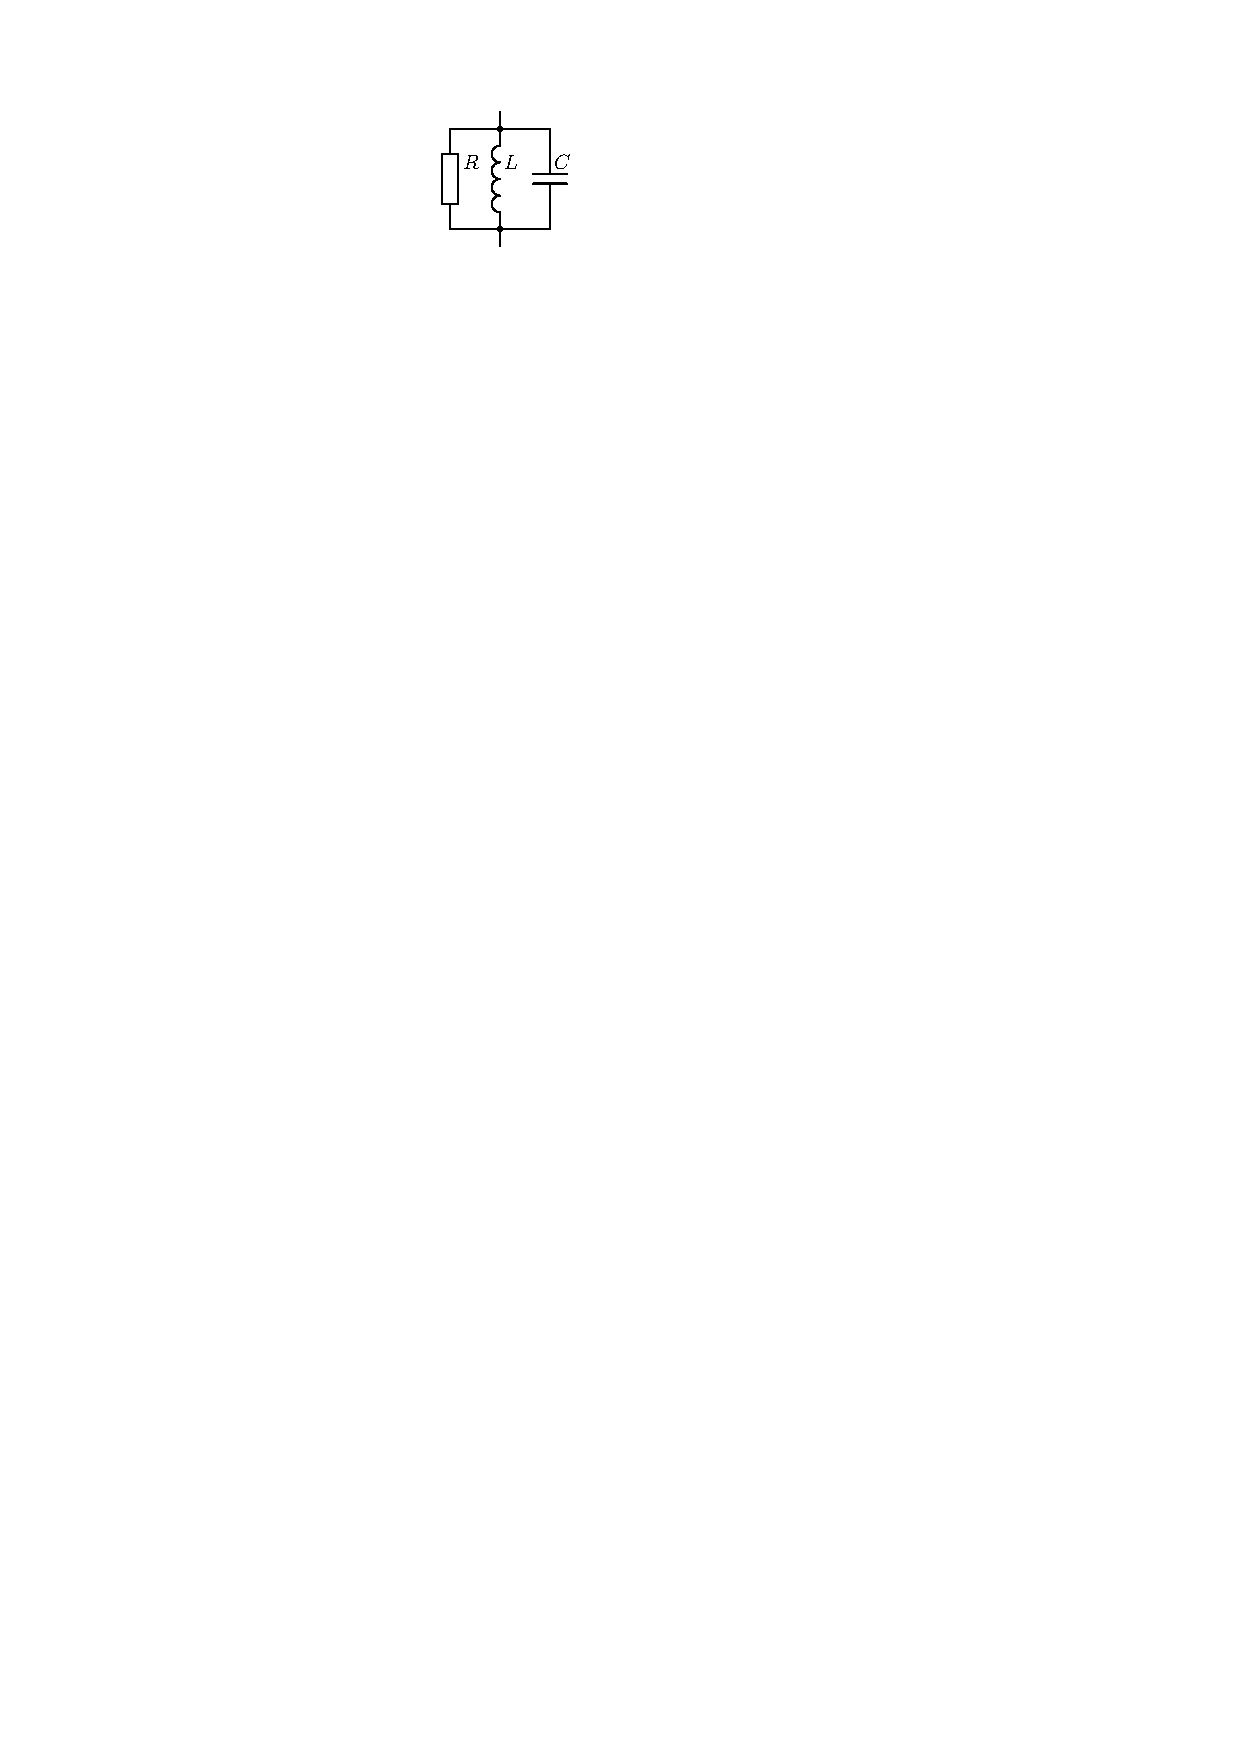
\includegraphics[scale=1.4]{./figs/RLC_circuit.pdf}
  \caption[Parallelschwingkreis als Modell für die elektrischen Eigenschaften eines Hohlraumresonators in der Nähe einer Resonanz]{Ein Parallelschwingkreis bestehend aus dem \textsc{ohm}schen Widerstand~$R$, der Induktivität~$L$ und der Kapazität~$C$ als Modell für die elektrischen Eigenschaften eines Hohlraumresonators in der Nähe einer Resonanz.}
  \label{fig:rlc_circuit}
\end{figure}
Die elektrischen Eigenschaften von Hohlraumresonatoren können in einem beschränkten Frequenzbereich um eine Resonanz durch das Modell des Parallelschwingkreises (siehe Abb.\ \ref{fig:rlc_circuit}) erklärt werden \cite[S.\ 179 f.]{wille}.
Zu dessen vollständiger Beschreibung ist die Angabe der drei Kenngrößen Widerstand~$R$, Induktivität~$L$ und Kapazität~$C$ ausreichend.
Für die Behandlung von Hohlraumresonatoren ist es zweckmäßig, andere Parameter zur Beschreibung zu wählen.
Daher verwendet man stattdessen die Eigenfrequenz~$\omega_0$, die Kreisgüte~$Q_0$ und der Widerstand~$R$ zur Charakterisierung des Schwingkreises.
Die Eigenfrequenz des Kreises folgt aus der \textsc{Thomson}schen Schwingungsgleichung
\begin{align}
  \omega_0 = \frac{1}{\sqrt{L C}}
\end{align}
und die Kreisgüte aus ihrer Definition
\begin{align}
  Q_0 &\coloneqq 2\pi \cdot \frac{\text{gespeicherte Energie}}{\text{Energieverlust pro Periode}} = \frac{\omega_0 W_0}{P_\mathrm{V}} = \omega_0 R C
  \label{eq:def_guete}
\end{align}
mit der im Kreis gespeicherten Energie $W_0$ und der Verlustleistung $P_\mathrm{V}$ aufgrund des \textsc{ohm}schen Widerstandes $R$.
Nach der Einführung dieser Kenngrößen kann die Impedanz $Z(\omega)$ des Kreises beziehungsweise des Hohlraumresonators ausgedrückt werden als
\begin{align}
  Z(\omega) = \left( \frac{1}{R} + \frac{1}{\I \omega L} + \I \omega C \right)^{-1} = \frac{R}{1 + \I Q_0 \left( \frac{\omega}{\omega_0}  - \frac{\omega_0}{\omega}\right)} \eqdot
\end{align}

Bisher war die Betrachtung auf ungetriebene Resonatoren beschränkt und soll nun auf die Anregung durch ein externes Hochfrequenzsignal erweitert werden.
Zur Übertragung dessen Leistung über einen angeschlossenen Wellenleiter mit charakteristischer Impedanz~$Z_0$ an eine Schwingungsmode der Kavität, können verschiedene Methoden verwendet werden.
Eine ist die induktive Kopplung an das Magnetfeld der Mode, bei der der Wellenleiter mit einer Leiterschleife (die sog.\ Koppelschleife) im Resonator verbunden ist.
Dadurch wird in der Leiterschleife ein hochfrequenter Wechselstrom angeregt, welcher ein zeitlich veränderliches Magnetfeld erzeugt. Dieses kann an das Magnetfeld verschiedener Moden der Kavität koppeln und diese anregen.
\begin{figure}[htb]
  \centering
  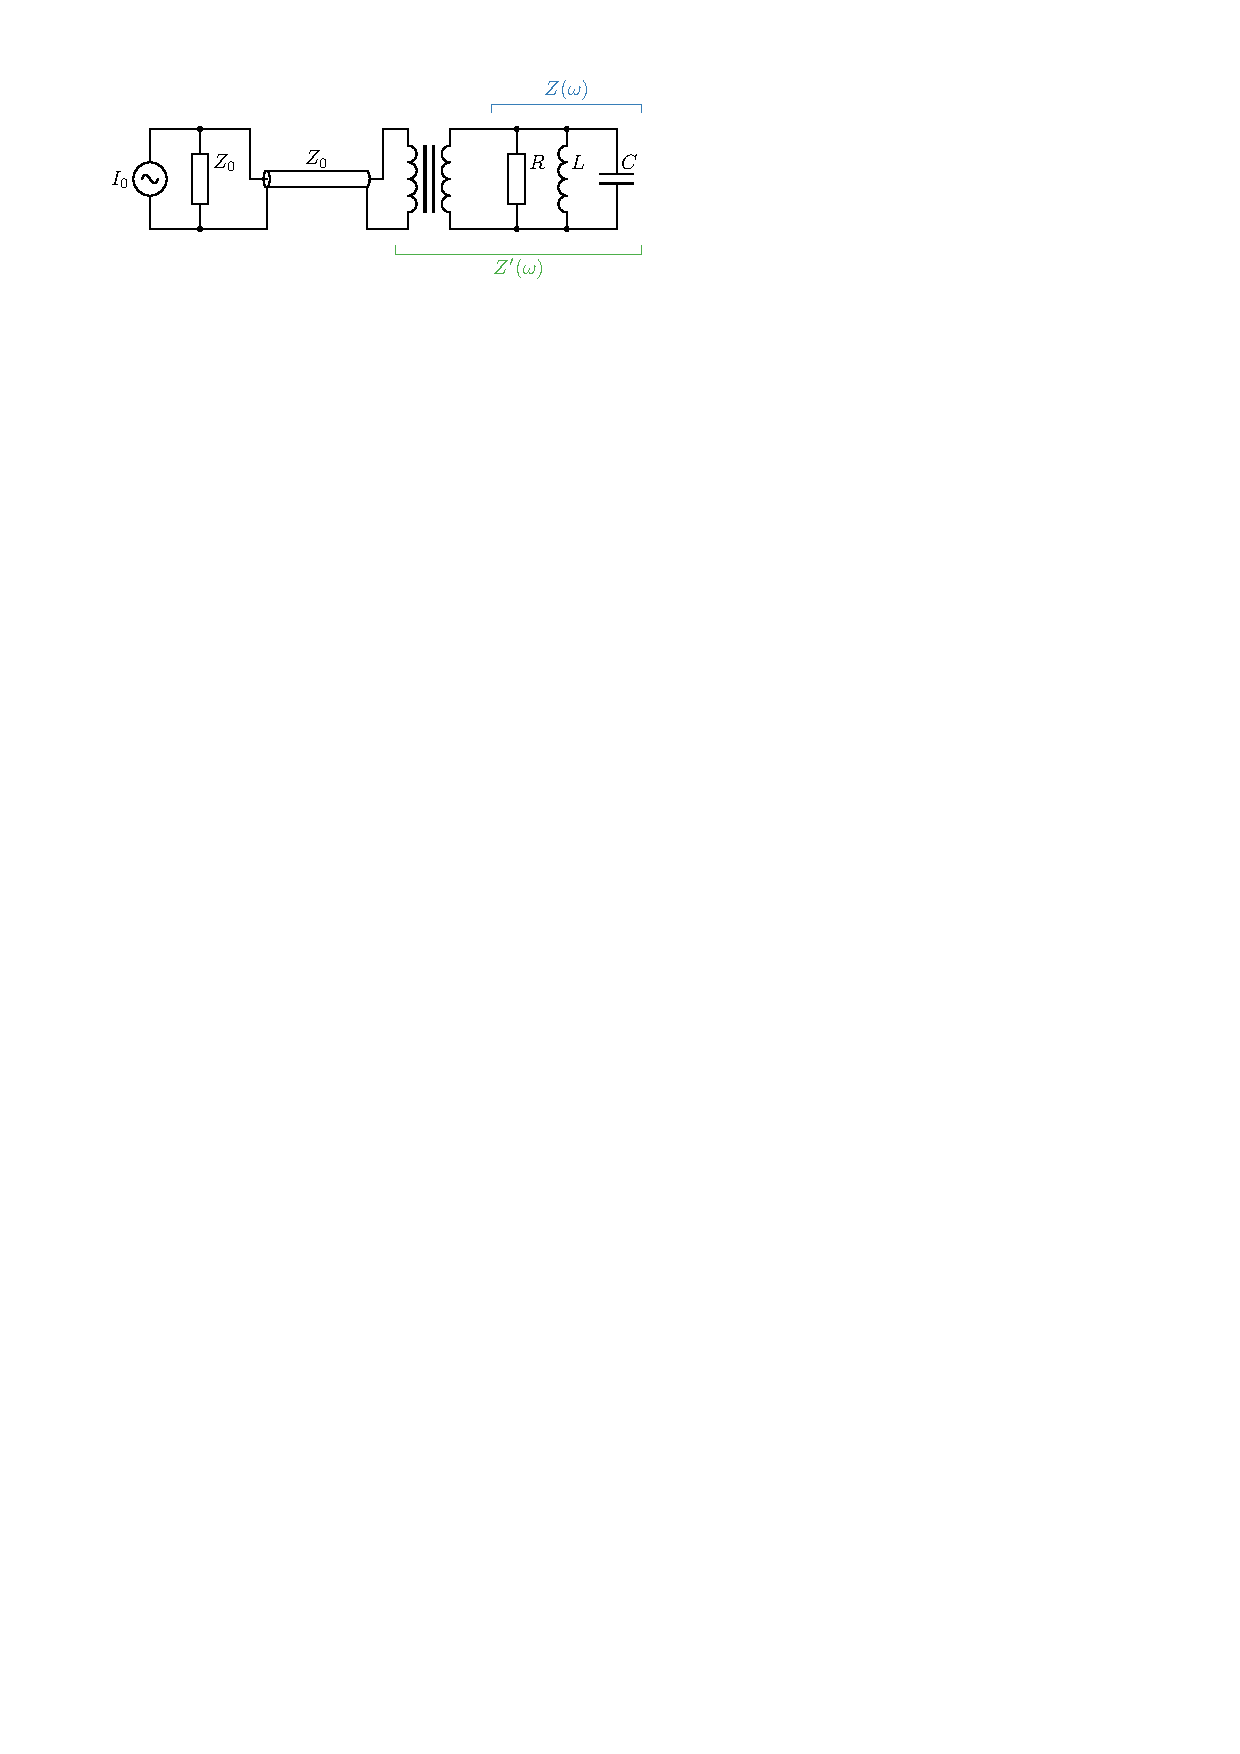
\includegraphics[scale=1.4]{./figs/RLC_coupling.pdf}
  \caption[Modell der induktiven Kopplung eines Hochfrequenzsignals über die Koppelschleife an den Resonator]{Modell der induktiven Kopplung eines treibenden Hochfrequenzsignals~$U_0$ über die Koppelschleife an den Resonator. Die Signalquelle ist mit einem Wellenleiter charakteristischer Impedanz~$Z_0$ mit der Koppelschleife verbunden. Die Impedanz des Resonators~$Z$ im Sekundärkreis wird durch die induktive Kopplung zur Impedanz~$Z^\prime$ im Primärkreis transformiert.}
  \label{fig:rlc_coupling}
\end{figure}

Im Modell des Parallelschwingkreises (vgl.\ Abb.\ \ref{fig:rlc_coupling}) bedeutet dies, dass die Impedanz~$Z(\omega)$ der Kavität durch die induktive Kopplung transformiert wird.
Direkt hinter der Koppelschleife habe der Resonator die transformierte Impedanz~$Z^\prime(\omega)$.
Man definiert als Maß für die Kopplung den sog.\ Koppelfaktor
\begin{align}
  \kappa \coloneqq \frac{Z^\prime(\omega_0)}{Z_0}
  \label{eq:koppelfaktor}
\end{align}
mit dem Wellenwiderstand~$Z_0$ des Wellenleiters und unterscheidet zwischen unterkritischer $(\kappa < 1)$, kritischer $(\kappa = 1)$ und überkritischer Kopplung $(\kappa > 1)$.
Im Falle von resonanter Anregung bei kritischer Kopplung folgert man aus Gleichung \eqref{eq:koppelfaktor}, dass der Wellenleiter mit seiner charakteristischen Impedanz abgeschlossen ist und somit keine Reflexionen an der Koppelschleife entstehen.
Mit der Definition des Koppelfaktors und der Proportionalität $Z^\prime(\omega) \propto Z(\omega)$ für ideale Transformatoren folgt die Frequenzabhängigkeit der Impedanz~$Z^\prime(\omega)$ des Systems bestehend aus Koppelschleife und Resonator:
\begin{align}
  Z^\prime(\omega) = \kappa \frac{Z_0}{R} Z(\omega) \eqdot
  \label{eq:impedanz_hinter_schleife}
\end{align}

Von besonderem Interesse ist der komplexe Reflexionskoeffizient zwischen Wellenleiter und Koppelschleife.
Er beschreibt das Verhältnis der komplexen Spannungsamplituden von hin- und rücklaufender Welle in einem Wellenleiter.
Aus der Leitungstheorie \cite[S.\ 57]{pozar} folgt für den Reflexionskoeffizienten~$\rho$ am Übergang von einem Wellenleiter mit Wellenwiderstand~$Z_0$ auf eine Abschlussimpedanz~$Z^\prime$:
\begin{align}
  \rho = \frac{Z^\prime - Z_0}{Z^\prime + Z_0} \eqdot
  \label{eq:reflexionskoeff_trans_line}
\end{align}
Es folgt nach Einsetzen von Gl.~\eqref{eq:impedanz_hinter_schleife} in Gl.~\eqref{eq:reflexionskoeff_trans_line} der Ausdruck für den Reflexionskoeffizienten:
\begin{align}
  \rho(\omega) = \frac{\frac{\kappa}{R} \cdot Z(\omega) - 1}{\frac{\kappa}{R} \cdot Z(\omega) + 1} = \frac{(\kappa - 1) + \I  Q_0 \left( \frac{\omega}{\omega_0}  - \frac{\omega_0}{\omega}\right)}{\left( \kappa + 1 \right) + \I  Q_0 \left( \frac{\omega}{\omega_0}  - \frac{\omega_0}{\omega}\right)}
  \label{eq:reflexionskoeff_komplex}
\end{align}
Betrachtet man außerdem den Absolutbetrag des Reflexionskoeffizienten
\begin{align}
  | \rho(\omega) | = \sqrt{\frac{(\kappa - 1)^2 + Q_0^2 \left( \frac{\omega}{\omega_0}  - \frac{\omega_0}{\omega}\right)^2}{(\kappa + 1)^2 + Q_0^2 \left( \frac{\omega}{\omega_0}  - \frac{\omega_0}{\omega}\right)^2}} \eqcomma
  \label{eq:resonanzkurve}
\end{align}
so ergeben sich charakteristische Resonanzkurven, wie in Abbildung \ref{fig:resonanzkurve} für verschiedene Güten und Koppelfaktoren dargestellt.
\begin{figure}[h]
  \centering
  % GNUPLOT: LaTeX picture with Postscript
\begingroup
  \makeatletter
  \providecommand\color[2][]{%
    \GenericError{(gnuplot) \space\space\space\@spaces}{%
      Package color not loaded in conjunction with
      terminal option `colourtext'%
    }{See the gnuplot documentation for explanation.%
    }{Either use 'blacktext' in gnuplot or load the package
      color.sty in LaTeX.}%
    \renewcommand\color[2][]{}%
  }%
  \providecommand\includegraphics[2][]{%
    \GenericError{(gnuplot) \space\space\space\@spaces}{%
      Package graphicx or graphics not loaded%
    }{See the gnuplot documentation for explanation.%
    }{The gnuplot epslatex terminal needs graphicx.sty or graphics.sty.}%
    \renewcommand\includegraphics[2][]{}%
  }%
  \providecommand\rotatebox[2]{#2}%
  \@ifundefined{ifGPcolor}{%
    \newif\ifGPcolor
    \GPcolortrue
  }{}%
  \@ifundefined{ifGPblacktext}{%
    \newif\ifGPblacktext
    \GPblacktexttrue
  }{}%
  % define a \g@addto@macro without @ in the name:
  \let\gplgaddtomacro\g@addto@macro
  % define empty templates for all commands taking text:
  \gdef\gplbacktext{}%
  \gdef\gplfronttext{}%
  \makeatother
  \ifGPblacktext
    % no textcolor at all
    \def\colorrgb#1{}%
    \def\colorgray#1{}%
  \else
    % gray or color?
    \ifGPcolor
      \def\colorrgb#1{\color[rgb]{#1}}%
      \def\colorgray#1{\color[gray]{#1}}%
      \expandafter\def\csname LTw\endcsname{\color{white}}%
      \expandafter\def\csname LTb\endcsname{\color{black}}%
      \expandafter\def\csname LTa\endcsname{\color{black}}%
      \expandafter\def\csname LT0\endcsname{\color[rgb]{1,0,0}}%
      \expandafter\def\csname LT1\endcsname{\color[rgb]{0,1,0}}%
      \expandafter\def\csname LT2\endcsname{\color[rgb]{0,0,1}}%
      \expandafter\def\csname LT3\endcsname{\color[rgb]{1,0,1}}%
      \expandafter\def\csname LT4\endcsname{\color[rgb]{0,1,1}}%
      \expandafter\def\csname LT5\endcsname{\color[rgb]{1,1,0}}%
      \expandafter\def\csname LT6\endcsname{\color[rgb]{0,0,0}}%
      \expandafter\def\csname LT7\endcsname{\color[rgb]{1,0.3,0}}%
      \expandafter\def\csname LT8\endcsname{\color[rgb]{0.5,0.5,0.5}}%
    \else
      % gray
      \def\colorrgb#1{\color{black}}%
      \def\colorgray#1{\color[gray]{#1}}%
      \expandafter\def\csname LTw\endcsname{\color{white}}%
      \expandafter\def\csname LTb\endcsname{\color{black}}%
      \expandafter\def\csname LTa\endcsname{\color{black}}%
      \expandafter\def\csname LT0\endcsname{\color{black}}%
      \expandafter\def\csname LT1\endcsname{\color{black}}%
      \expandafter\def\csname LT2\endcsname{\color{black}}%
      \expandafter\def\csname LT3\endcsname{\color{black}}%
      \expandafter\def\csname LT4\endcsname{\color{black}}%
      \expandafter\def\csname LT5\endcsname{\color{black}}%
      \expandafter\def\csname LT6\endcsname{\color{black}}%
      \expandafter\def\csname LT7\endcsname{\color{black}}%
      \expandafter\def\csname LT8\endcsname{\color{black}}%
    \fi
  \fi
    \setlength{\unitlength}{0.0500bp}%
    \ifx\gptboxheight\undefined%
      \newlength{\gptboxheight}%
      \newlength{\gptboxwidth}%
      \newsavebox{\gptboxtext}%
    \fi%
    \setlength{\fboxrule}{0.5pt}%
    \setlength{\fboxsep}{1pt}%
\begin{picture}(3400.00,2124.00)%
    \gplgaddtomacro\gplbacktext{%
    }%
    \gplgaddtomacro\gplfronttext{%
      \csname LTb\endcsname%
      \put(176,1116){\rotatebox{-270}{\makebox(0,0){\strut{}$|\rho|$}}}%
      \put(1699,154){\makebox(0,0){\strut{}$\omega$}}%
      \csname LTb\endcsname%
      \put(2091,285){\makebox(0,0){\strut{}\scriptsize{$\omega_0$}}}%
      \put(1700,775){\makebox(0,0){\strut{}$\Delta \omega$}}%
      \put(1308,285){\makebox(0,0){\strut{}\scriptsize{$\omega_1$}}}%
    }%
    \gplbacktext
    \put(0,0){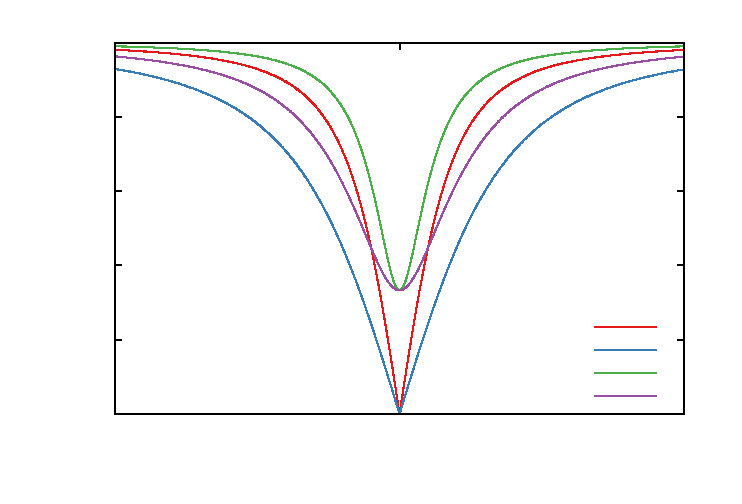
\includegraphics{./plots/resonanzkurve}}%
    \gplfronttext
  \end{picture}%
\endgroup

  \caption[Verhalten des Reflexionskoeffizienten $|\rho|$ für Resonanzen verschiedener Güten~$Q_0$ und Koppelfaktoren~$\kappa$]{Verhalten des Reflexionskoeffizienten $|\rho|$ in Abhängigkeit der auf die Resonanzfrequenz normierten Frequenz~$\frac{\omega}{\omega_0}$ für Resonanzen verschiedener Güten~$Q_0$ und Koppelfaktoren~$\kappa$.}
  \label{fig:resonanzkurve}
\end{figure}
Diese Gleichungen ermöglichen den experimentellen Zugang zur Bestimmung von Koppelfaktor~$\kappa$, Güte~$Q_0$ und Resonanzfrequenz~$\omega_0$ von Hohlraumresonatoren.


%------------------------------------------------------------------------------
\section{Resonante Störkörpermessung}
\label{sec:resonante_stoerkoerpermessung}
%------------------------------------------------------------------------------
Die resonante Störkörpermessung dient der Bestimmung der ortsabhängigen elektrischen und magnetischen Feldamplituden in Hohlraumresonatoren.
Sie basiert auf der Störung des elektromagnetischen Feldes im Resonatorinnenraum durch einen dielektrischen oder magnetischen Körper (dem sog.\ Störkörper), welcher durch das Feld polarisiert beziehungsweise magnetisiert wird.
Eine solche lokalisierte Störung verursacht eine Verschiebung der Resonanzfrequenz~$\Delta \omega$ in Abhängigkeit des elektrischen und magnetischen Feldes am Ort des Störkörpers.
Quantitativ kann die Verschiebung beschrieben werden durch (für eine Herleitung siehe Anhang \ref{app:herleitung_frequenzverschiebung}):
\begin{align}
  \frac{\Delta \omega}{\omega_0} = - \frac{\int_V \mathrm{d}V \left[ \ve_0^* \cdot \vec{P} + \vb_0^* \cdot \vec{M} \right]}{4 W_0}
  \label{eq:frequenzverschiebung}
\end{align}
wobei $V$ das Resonatorvolumen, $\vec{P}$ die Polarisation, $\vec{M}$ die Magnetisierung, $W_0$ die im elektromagnetischen Feld gespeicherte Energie und $\ve_0^*, \vb_0^*$ die komplex konjugierten Felder des ungestörten Resonators sind.

Im Rahmen dieser Arbeit wird eine dielektrische Kugel mit relativer elektrischer Permittivität~$\varepsilon_\mathrm{r}$ verwendet.
Darüber hinaus sei die relative magnetische Permeabilität des Störkörpers $\mu_\mathrm{r} = 1$, sodass die Magnetisierung im externen Feld vernachlässigt werden kann.
Weiterhin wird angenommen, dass das Volumen des kugelförmigen Störkörpers wesentlich kleiner ist als das Resonatorvolumen, sodass am Ort des Störkörpers das elektrische Feld als homogen angesehen werden kann.
Dadurch kann die Polarisation $\vec{P}$ der dielektrischen Kugel im homogenen elektrischen Feld $\ve_0$ ausgedrückt werden als \cite[S.\ 115]{jackson}:
\begin{align}
  \vec{P} = 3 \, \frac{\varepsilon_\mathrm{r} - 1}{\varepsilon_\mathrm{r} + 2} \, \varepsilon_0 \ve_0
  \label{eq:polarisation_kugel}
\end{align}
mit der elektrischen Feldkonstante~$\varepsilon_0$.
Durch die Annahme der Homogenität der Felder am Ort des Störkörpers und verschwindender Polarisation und Magnetisierung außerhalb des Störkörpervolumens~$V_\mathrm{s}$, kann von der Integration über das Resonatorvolumen~$V$ in Gleichung \eqref{eq:frequenzverschiebung} zur Integration über das Störkörpervolumen übergangen werden.
Nach Einsetzen der Polarisation der dielektrischen Kugel in Gleichung \eqref{eq:frequenzverschiebung} folgt für die Amplitude des elektrischen Feldes am Ort des Störkörpers $|\ve_0(x_\mathrm{s}, y_\mathrm{s}, z_\mathrm{s})|$:
\begin{align}
  |\ve_0(x_\mathrm{s}, y_\mathrm{s}, z_\mathrm{s})| = \sqrt{-4 \cdot \frac{W_0}{\alpha_\mathrm{s}} \cdot \frac{\Delta \omega}{\omega_0}} \qquad \text{mit} \qquad \Delta \omega \leq 0
  \label{eq:skm_e_feld}
\end{align}
(folglich durch $|\ve_0|$ abgekürzt) und der Störkörperkonstanten~$\alpha_\mathrm{s}$ für sphärische Störkörper:
\begin{align}
  \alpha_\mathrm{s} \coloneqq 3 \, \frac{\varepsilon_\mathrm{r} - 1}{\varepsilon_\mathrm{r} + 2} \, \varepsilon_0 V_\mathrm{s} \eqdot
  \label{eq:stoerkoerperkonstante}
\end{align}
Um die Amplitude des elektrischen Feldes unabhängig von der im Resonator gespeicherten Energie~$W_0$ angeben zu können, verwendet man die Definition der Güte~$Q_0$ in Gleichung \eqref{eq:def_guete} und normiert das elektrische Feld auf die Wurzel der Verlustleistung~$P_\mathrm{V}$ des Resonators:
\begin{align}
  \frac{|\ve_0|}{\sqrt{P_\mathrm{V}}} = \sqrt{-4 \cdot \frac{Q_0}{\alpha_s} \cdot \frac{\Delta \omega}{\omega_0^2}}
  \label{eq:skm_e_feld_normiert}
\end{align}
Diese Größe ist unabhängig von der in den Resonator eingekoppelten Leistung und dient als Basis für die folgenden Berechnungen.


%------------------------------------------------------------------------------
\section{Charakteristische Größen von Beschleunigungsresonatoren}
\label{sec:resonator_charakteristiken}
%------------------------------------------------------------------------------
Eine wichtige Kenngrößen von Moden in Beschleunigungsresonatoren ist die Beschleunigungsspannung~$U$, die ein Teilchen erfährt, das einen Resonator der Länge~$L$ instantan durchquert:
\begin{align}
  U = \int_0^L |\ve_0 (z)| \, \mathrm{d}z \eqdot
  \label{eq:beschleunigungsspannung}
\end{align}
Um den effektiven Energiegewinn eines Teilchens zu erhalten, muss die endliche Geschwindigkeit des Teilchens und die harmonische Zeitabhängigkeit des Feldes beachtet werden.
Dazu definiert man den Laufzeitfaktor~$\Lambda$ für ultrarelativistische Teilchen ($v = c$):
\begin{align}
  \Lambda = \left| \frac{ \int_0^L |\ve_0(z)| \cdot \sin\left( \frac{\omega_0}{c} z + \varphi_0 \right) \, \mathrm{d}z }{ \int_0^L |\ve_0(z)| \, \mathrm{d}z } \right| \eqcomma
  \label{eq:laufzeitfaktor}
\end{align}
wobei die Phase $\varphi_0$ so zu wählen ist, dass der Laufzeitfaktor maximiert wird.
Dadurch erhält man die effektive Beschleunigungsspannung~$U_\mathrm{eff}$:
\begin{align}
  U_\mathrm{eff} = \Lambda \cdot U
  \label{eq:eff_beschleunigungsspannung}
\end{align}
und damit die Änderung der Energie eines ultrarelativistischen Teilchens der Ladung $q$ beim Passieren des Resonators $\Delta E = q \cdot U_\mathrm{eff}$.
Darüber hinaus definiert man als Maß für die Effizienz der Beschleunigung die sog.\ Shuntimpedanz~$R_\mathrm{S}$:
\begin{align}
  R_\mathrm{S} = \frac{U^2}{2 P_\mathrm{V}}
  \label{eq:shuntimpedanz}
\end{align}
mit der in den Resonatorwänden dissipierten Leistung $P_\mathrm{V}$ und analog die effektive Shuntimpedanz~$R_\mathrm{S}^\mathrm{eff}$:
\begin{align}
  R_\mathrm{S}^\mathrm{eff} = \frac{U_\mathrm{eff}^2}{2 P_\mathrm{V}} = \Lambda^2 \cdot R_\mathrm{S} \eqdot
  \label{eq:eff_shuntimpedanz}
\end{align}
In Abhängigkeit der im Resonator angeregten Moden unterscheidet man zwischen longitudinaler und transversaler Beschleunigungsspannung/Shuntimpedanz.
Dies liegt darin begründet, dass TM-Moden nur elektrische Felder mit longitudinaler und TE-Moden mit transversaler Ausrichtung aufweisen und dementsprechend nur zur longitudinalen/transversalen Beschleunigung der Teilchen führen.

\todo{Verlustfaktor?, R/Q, R/(Q*L), Resonanzkurve und charakteristische Eigenschaften, mehr mit Zitaten hinterlegen}
%$R$ über $Q_0$\footnote{Unabhängig von Verlusten, nur Geometrieabhängig}: $R_\mathrm{S}/Q_0$
